\begin{figure}[ht] 
 	\centering 
 	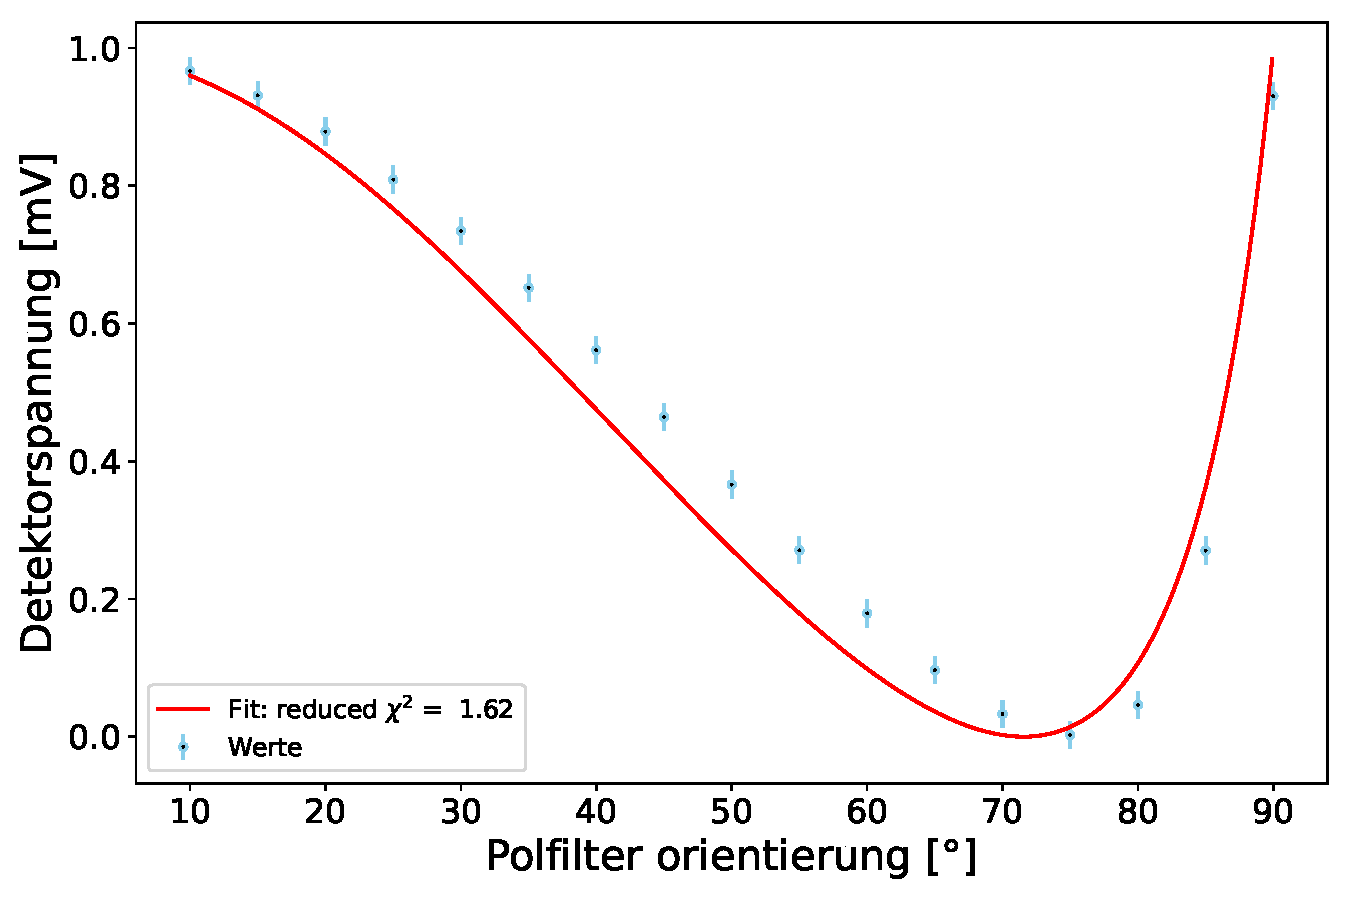
\includegraphics[width= 0.65 \textwidth]{Fits/Rp_Rs_Si_Fit.pdf} 
	\caption{Rp_Rs_Si, Fit} 
 	\label{fig:Rp_Rs_Si, Fit} 
\end{figure}
 \\ 
\begin{align} 
 	 f(x) = a x^{4} + b x^{3} + c x^{2} + d x + e
\end{align} 
\begin{table}[ht] 
\centering 
\caption{Rp_Rs_Si, Fit Parameter Tabelle} 
\label{tab:my-table}
\begin{tabular}{|l|c|}
\hline
Parameter Name	&	Wert \\ \hline
n	&	 3.000 \pm  0.327\\ \hline
kappa	&	 0.00 \pm  55739.301\\ \hline
\end{tabular} 
\end{table}